% \input{Figures/ode-sde-vpsde/svdd}

% 
% 
\vspace{-0.6\baselineskip}
\section{Applications}
\vspace{-0.6\baselineskip}
\label{sec:applications}
In this section, we present the experimental results of particle sampling methods for inference-time reward alignment. 
In Appendix, we present i) implementation details of the search algorithms, ii) aesthetic image generation, iii) comparisons between diffusion and flow models, iv) scaling behavior comparison of Best-of-N (BoN) and \Ours{}, and v) additional qualitative results. 
% 
\vspace{-0.3\baselineskip}
\subsection{Experiment Setup} 
\vspace{-0.3\baselineskip}
\paragraph{Tasks.}
In this section, we present the results for the following applications: compositional text-to-image generation and quantity-aware image generation, where the rewards are non-differentiable. 
For the differentiable reward case, we consider aesthetic image generation (Appendix~\ref{sec:appendix_diff_reward}). 
% The goal of compositional text-to-image generation is to generate images that faithfully represent complex textual descriptions while ensuring the correct integration of attributes and logical relationships. 
In compositional text-to-image generation, we use all $121$ text prompts from GenAI-Bench~\cite{Jiang:2024GenAI} that contain three or more advanced compositional elements. 
% We use all $121$ text prompts containing three or more compositional elements from GenAI-Bench~\cite{Jiang:2024GenAI}. 
For quantity-aware image generation, we use $100$ randomly sampled prompts from T2I-CompBench++~\cite{Huang:2025T2ICompBench++} numeracy category. 
% produces images that precisely match the specified quantities and categories of objects in the given text prompts. We use $100$ randomly sampled prompts from T2I-CompBench++~\cite{Huang:2025T2ICompBench++}. 

For all applications, we use FLUX~\cite{BlackForestLabs:2024Flux} as the pretrained flow model. We fix the total number of function evaluations (NFEs) to $500$ and set the number of denoising steps to $10$, which allocates $50$ NFEs per denoising step. As a reference, we also include the results of the base pretrained models without inference-time scaling. Additionally, we present a comparison between flow models and diffusion models in Appendix~\ref{sec:appendix_diff_flow}. 
% 
% 
\vspace{-0.5\baselineskip}
\paragraph{Baselines.} We evaluate inference-time search algorithms discussed in Sec.~\ref{sec:related}, including Best-of-N (BoN), Search over Paths (SoP)~\cite{Ma2025:SoP}, SMC~\cite{Kim:2025DAS}, CoDe~\cite{Singh:2025CoDE}, and SVDD~\cite{Li2024:SVDD}. 
We categorize BoN and SoP as Linear-ODE-based methods, as their generative processes follow the deterministic process in Eq.~\ref{eq:pf-ode}. 
For SMC, we adopt DAS~\cite{Kim:2025DAS}; however, when the reward is non-differentiable, we use the reverse transition kernel of the pretrained model as the proposal distribution. 


\begin{figure}[t]
    \definecolor{YellowGreen}{RGB}{49,126,53}
    \definecolor{Rhodamine}{RGB}{243,156,146}
    \definecolor{Dandelion}{RGB}{242,193,106}
    \vspace{-0.5\baselineskip}
    \centering
    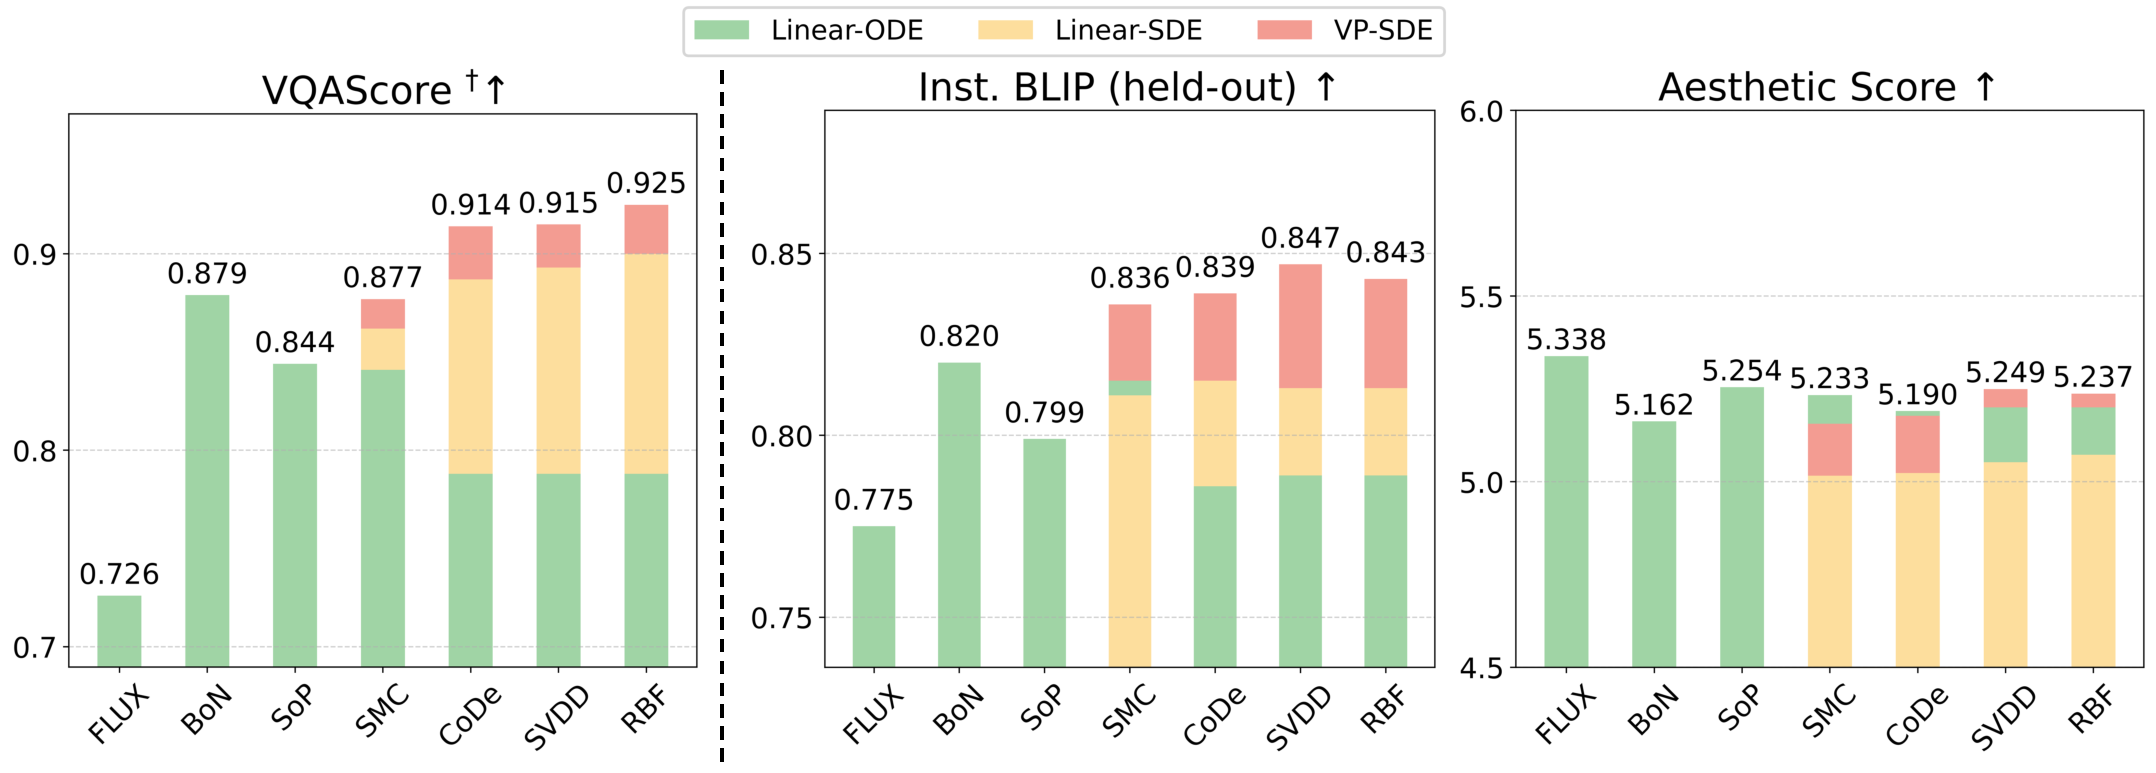
\includegraphics[width=1.0\linewidth]{Tables/compo_bar_graph/compo_bar_graph.pdf}
    \caption{\textbf{Quantitative results of compositional text-to-image generation.} \textsuperscript{\textdagger} denotes the given reward used in inference-time scaling (left). 
    Notably, performance consistently improves from {\color{YellowGreen}Linear-ODE} to {\color{Dandelion}Linear-SDE} and {\color{Rhodamine}VP-SDE} for both given and held-out rewards (left, middle), without significant quality degradation, as evidenced by the comparable aesthetic score~\cite{Schuhmann:aesthetics} (right).} 
    \label{fig:composition_main}
    \vspace{-0.75\baselineskip}
\end{figure}

% \begin{table*}[!t]
% \setlength{\tabcolsep}{1.5pt}
% \centering
% \scriptsize
% \renewcommand{\arraystretch}{1.2} 
% \caption{\textbf{Quantitative results of compositional image generation.} \textsuperscript{\textdagger} denotes the given reward used in inference-time scaling. The best result in the given and held-out reward is highlighted by \textbf{bold}, and the runner-up is \underline{underlined}. L.O., L.S., and V.S. indicate Linear-ODE, Linear-SDE, and VP-SDE.}
% \vspace{-0.5\baselineskip}
% \label{tab:composition_main}
% \newcolumntype{X}{>{\centering\arraybackslash}m{0.13\linewidth}}
% \newcolumntype{Y}{>{\centering\arraybackslash}m{0.065\linewidth}}
% \newcolumntype{W}{>{\centering\arraybackslash}m{0.045\linewidth}}
% \begin{tabular}{X | Y Y Y | W W W | W W W | W W W | W W W }
% \toprule
% \multirow{2}{*}{Metric} & 
% \multirow{1}{*}{\makecell{FLUX~\cite{BlackForestLabs:2024Flux}}} & 
% \multirow{1}{*}{BoN} & 
% \multirow{1}{*}{\makecell{SoP~\cite{Ma2025:SoP}}} & 
% \multicolumn{3}{c|}{SMC~\cite{Kim:2025DAS}} & 
% \multicolumn{3}{c|}{CoDe~\cite{Singh:2025CoDE}} & 
% \multicolumn{3}{c|}{SVDD~\cite{Li2024:SVDD}} & 
% \multicolumn{3}{c}{{\Oursbf{}} (Ours)} \\
% \cline{2-16}
% & \multicolumn{3}{c|}{L.O.} & L.O. & L.S. & V.S. & L.O. & L.S. & V.S. & L.O. & L.S. & V.S. & L.O. & L.S. & V.S. \\
% \hline
% \makecell{VQAScore\textsuperscript{\textdagger}\\\cite{Lin:2024CLIPFlanT5}~$\uparrow$} & 
% 0.726 & 0.879 & 0.844 & 
% 0.841 & 0.862 & 0.877 & 
% 0.788 & 0.887 & 0.914 & 
% 0.788 & 0.893 & \underline{0.915} & 
% 0.788 & 0.900 & \textbf{0.925} \\
% \hline
% Inst. BLIP~\cite{Dai:2023InstructBLIP}~$\uparrow$ (held-out) & 
% 0.775 & 0.820 & 0.799 & 
% 0.815 & 0.811 & 0.836 & 
% 0.786 & 0.815 & 0.839 & 
% 0.789 & 0.813 & \textbf{0.847} & 
% 0.789 & 0.813 & \underline{0.843} \\
% \hline
% Aesthetic Score~\cite{Schuhmann:aesthetics}~$\uparrow$ & 
% 5.338 & 5.162 & 5.254 & 
% 5.233 & 5.016 & 5.156 & 
% 5.190 & 5.023 & 5.177 & 
% 5.200 & 5.052 & 5.249 & 
% 5.200 & 5.072 & 5.237 \\
% \bottomrule
% \end{tabular}
% \vspace{-0.75\baselineskip}
% \end{table*}




% =============================================================================== %
% Multicolumn Multirow error in cline.
% \begin{table*}[!t]
%     \setlength{\tabcolsep}{1.5pt}
%     \centering
%     \scriptsize
%     \newcommand{\good}[1]{\tiny{\textcolor{blue}{+#1\%}}}
%     \newcommand{\bad}[1]{\tiny{\textcolor{red}{-#1\%}}}
%     \caption{\textbf{Quantitative results of compositional image generation.} \textsuperscript{\textdagger} denotes the given reward used in inference-time scaling. For particle-based sampling methods, the relative improvement in each cell is computed with respect to the Linear-ODE case. The best result in the given and held-out reward is highlighted by \textbf{bold}, and the runner-up is \underline{underlined}. L.O., L.S., and V.S. indicate Linear-ODE, Linear-SDE, and VP-SDE, respectively. \textsuperscript{*} denotes results with $50$ denoising steps.}
%     \vspace{-0.5\baselineskip}
%     \label{tab:composition_main}
%     \newcolumntype{X}{>{\centering\arraybackslash}m{0.12\linewidth}}
%     \newcolumntype{Y}{>{\centering\arraybackslash}m{0.04\linewidth}}
%     \newcolumntype{W}{>{\centering\arraybackslash}m{0.06\linewidth}}
%     \begin{tabular}{X | W W W | W Y Y | W Y Y | W Y Y | W Y Y }
%         \toprule
%         \multirow{2}{*}{\makecell{Metric}} & 
%         \multirow{2}{*}{FLUX} & \multirow{2}{*}{BoN} & \multirow{2}{*}{\makecell{SoP~\cite{Ma2025:SoP}}} & \multicolumn{3}{c|}{\multirow{2}{*}{SMC~\cite{Kim:2025DAS}}} & \multicolumn{3}{c|}{\multirow{2}{*}{CoDe~\cite{Singh:2025CoDE}}} & \multicolumn{3}{c|}{\multirow{2}{*}{SVDD~\cite{Li2024:SVDD}}} & \multicolumn{3}{c}{\multirow{2}{*}{{\Oursbf{}} (Ours)}} \\
%         \cline{2-16}
%         & \multicolumn{3}{c|}{L.O.} & L.O. & L.S. & V.S. & L.O. & L.S. & V.S. & L.O. & L.S. & V.S. & L.O. & L.S. & V.S. \\
%         \hline
%         \makecell{VQAScore\textsuperscript{\textdagger}\\\cite{Lin:2024CLIPFlanT5} $\uparrow$} & 0.726 & 0.879 & 0.844 & 0.841 & \makecell{0.862} & \makecell{0.877} & 0.788 & \makecell{0.887} & \makecell{0.914} & 0.788 & \makecell{0.893} & \makecell{\underline{0.915}} & 0.788 & \makecell{0.900} & \makecell{\textbf{0.925}} \\
%         \hline
%         \makecell{Inst. BLIP~\cite{Dai:2023InstructBLIP} $\uparrow$ \\ (held-out)} & 0.775 & 0.820 & 0.799 & 0.815 & \makecell{0.811} & \makecell{0.836} & 0.786 & \makecell{0.815} & \makecell{0.839} & 0.789 & \makecell{0.813} & \makecell{\textbf{0.847}} & 0.789 & \makecell{0.813} & \makecell{\underline{0.843}} \\
%         \hline
%         \makecell{Aesthetic \\ Score~\cite{Schuhmann:aesthetics} $\uparrow$} & 5.338 & 5.162 & 5.254 & 5.233 & 5.016 & 5.156 & 5.190 & 5.023 & 5.177 & 5.200 & 5.052 & 5.249 & 5.200 & 5.072 & 5.237 \\
%         \bottomrule
%     \end{tabular}
%     \vspace{-0.25\baselineskip}
% \end{table*}



% % =============================================================================== %
% % ===================== 3/8 16:47 Juil's Update ================================= %
% % =============================================================================== %
% \begin{table*}[!t]
%     \setlength{\tabcolsep}{1.5pt}
%     \centering
%     \scriptsize
%     \newcommand{\good}[1]{\tiny{\textcolor{blue}{+#1\%}}}
%     \newcommand{\bad}[1]{\tiny{\textcolor{red}{-#1\%}}}
%     \caption{\textbf{Quantitative results of compositional image generation.} \textsuperscript{\textdagger} denotes the given reward used in inference-time scaling. For particle-based sampling methods, the relative improvement in each cell is computed with respect to the Linear-ODE case. The best result in the given and held-out reward is highlighted by \textbf{bold}, and the runner-up is \underline{underlined}. L.O., L.S., and V.S. indicate Linear-ODE, Linear-SDE, and VP-SDE, respectively. \textsuperscript{*} denotes results with $50$ denoising steps.}
%     \vspace{-1.0\baselineskip}
%     \label{tab:composition_main}
%     \newcolumntype{X}{>{\centering\arraybackslash}m{0.095\linewidth}}
%     \newcolumntype{Y}{>{\centering\arraybackslash}m{0.045\linewidth}}
%     \newcolumntype{Z}{>{\centering\arraybackslash}m{0.05\linewidth}}
%     \newcolumntype{W}{>{\centering\arraybackslash}m{0.035\linewidth}}
%     \begin{tabular}{X | Y Y | Z Z | W W W | W Y Y | W Y Y | W Y Y | W Y Y }
%         \toprule
%         \multirow{4}{*}{\makecell{Metric}} & \multicolumn{4}{c|}{\textbf{Diffusion Model}} & \multicolumn{15}{c}{\textbf{Flow Model}} \\
%         \cline{2-20}
%         & \multirow{2}{*}{SD2} & \multirow{2}{*}{$\text{SD2}^{*}$} & \multicolumn{2}{c|}{SVDD~\cite{Li2024:SVDD}} & \multirow{2}{*}{FLUX} & \multirow{2}{*}{BoN} & \multirow{2}{*}{\makecell{SoP\\\cite{Ma2025:SoP}}} & \multicolumn{3}{c|}{\multirow{2}{*}{SMC~\cite{Kim:2025DAS}}} & \multicolumn{3}{c|}{\multirow{2}{*}{CoDe~\cite{Singh:2025CoDE}}} & \multicolumn{3}{c|}{\multirow{2}{*}{SVDD~\cite{Li2024:SVDD}}} & \multicolumn{3}{c}{\multirow{2}{*}{{\Oursbf{}} (Ours)}}\\
%         & & & SD2 & SD2$^{*}$ & & & & & & & & & & & & & & \\
%         % & \multirow{2}{*}{\makecell{SD}} & \multirow{2}{*}{\makecell{$\text{SD}^{*}$}} & \multicolumn{2}{c}{SVDD~\cite{Li2024:SVDD}} & \multirow{2}{*}{FLUX} & \multirow{2}{*}{BoN} & \multirow{2}{*}{SoP~\cite{Ma2025:SoP}} & \multirow{2}{*}{\multicolumn{3}{c|}}{\makecell{SMC \\ \cite{Kim:2025DAS}}} & \multirow{2}{*}{\multicolumn{3}{c|}{\makecell{CoDe \\ \cite{Singh:2025CoDE}}}} & \multirow{2}{*}{\multicolumn{3}{c|}{\makecell{SVDD\\\cite{Li2024:SVDD}}}} & \multirow{2}{*}{\multicolumn{3}{c}}{\makecell{{\Oursbf{}} (Ours)}} \\
        
%         % & \makecell{SD \\ \cite{Rombach:2022LDM}} & \makecell{$\text{SD}^{*}$ \\ \cite{Rombach:2022LDM}} & \makecell{SVDD \\ SD~\cite{Li2024:SVDD}} & \makecell{SVDD \\$\text{SD}^{*}$ \cite{Li2024:SVDD}} & \makecell{FLUX \\ \cite{BlackForestLabs:2024Flux}} & BoN & \makecell{SoP \\ \cite{Ma2025:SoP}} & \multicolumn{3}{c|}{\makecell{SMC \\ \cite{Kim:2025DAS}}} & \multicolumn{3}{c|}{\makecell{CoDe \\ \cite{Singh:2025CoDE}}} & \multicolumn{3}{c|}{\makecell{SVDD \\ \cite{Li2024:SVDD}}} & \multicolumn{3}{c}{\makecell{{\Oursbf{}} (Ours)}} \\
%         \cline{2-20}
%         & \multicolumn{2}{c|}{V.S.} & \multicolumn{2}{c|}{V.S.} & \multicolumn{3}{c|}{L.O.} & L.O. & L.S. & V.S. & L.O. & L.S. & V.S. & L.O. & L.S. & V.S. & L.O. & L.S. & V.S. \\
%         \hline
%         \makecell{VQAScore\textsuperscript{\textdagger}\\\cite{Lin:2024CLIPFlanT5} $\uparrow$} & 0.671 & 0.647 & 0.867 & 0.886 & 0.726 & 0.879 & 0.844 & 0.841 & \makecell{0.862\\\good{2.50}} & \makecell{0.877\\\good{4.28}} & 0.788 & \makecell{0.887\\\good{12.56}} & \makecell{0.914\\\good{15.99}} & 0.788 & \makecell{0.893\\\good{13.32}} & \makecell{\underline{0.915}\\\good{16.12}} & 0.788 & \makecell{0.900\\\good{14.21}} & \makecell{\textbf{0.925}\\\good{17.39}} \\
%         \hline
%         \makecell{Inst. BLIP~\cite{Dai:2023InstructBLIP} $\uparrow$ \\ (held-out)} & 0.741 & 0.739 & 0.790 & 0.799 & 0.775 & 0.820 & 0.799 & 0.815 & \makecell{0.811\\\bad{-0.49}} & \makecell{0.836\\\good{2.58}} & 0.786 & \makecell{0.815\\\good{3.69}} & \makecell{0.839\\\good{6.74}} & 0.789 & \makecell{0.813\\\good{3.04}} & \makecell{\textbf{0.847}\\\good{7.35}} & 0.789 & \makecell{0.813\\\good{3.04}} & \makecell{\underline{0.843}\\\good{6.84}} \\
%         \hline
%         \makecell{Aesthetic \\ Score~\cite{Schuhmann:aesthetics} $\uparrow$} & 5.107 & 5.115 & 5.181 & 5.213 & 5.338 & 5.162 & 5.254 & 5.233 & 5.016 & 5.156 & 5.190 & 5.023 & 5.177 & 5.200 & 5.052 & 5.249 & 5.200 & 5.072 & 5.237 \\
%         \toprule
%     \end{tabular}
%     \vspace{-0.25\baselineskip}
% \end{table*}

% =============================================================================== %
% ===================== 3/8 16:47 (Previous Version Juil Not Touched ============ %
% =============================================================================== %
% \begin{table*}[!t]
%     \setlength{\tabcolsep}{1.5pt}
%     \centering
%     \scriptsize
%     \newcommand{\good}[1]{\tiny{\textcolor{red}{+#1\%}}}
%     \newcommand{\bad}[1]{\tiny{\textcolor{blue}{-#1\%}}}
%     \caption{\textbf{Quantitative results of compositional image generation.} \textsuperscript{\textdagger} denotes the given reward used in inference time. For particle-based sampling methods, the relative improvement in each cell is computed w.r.t. the Linear-ODE. The best result in the given and held-out reward is highlighted by \textbf{bold}, and the runner-up is \underline{underlined}. L.O., L.S., and V.S. indicate Linear-ODE, Linear-SDE, and VP-SDE, respectively.}
%     \vspace{-1.0\baselineskip}
%     \label{tab:composition_main}
%     \newcolumntype{X}{>{\centering\arraybackslash}m{0.095\linewidth}}
%     \newcolumntype{Y}{>{\centering\arraybackslash}m{0.045\linewidth}}
%     \newcolumntype{Z}{>{\centering\arraybackslash}m{0.05\linewidth}}
%     \newcolumntype{W}{>{\centering\arraybackslash}m{0.035\linewidth}}
%     \begin{tabular}{X | Y Y | Z Z | W W W | W Y Y | W Y Y | W Y Y | W Y Y }
%         \toprule
%         \multirow{3}{*}{\makecell{Metric}} & \multicolumn{19}{c}{\textbf{Methods}} \\
%         \cline{2-20}
%         & \multicolumn{4}{c|}{\textbf{Diffusion Model}} & \multicolumn{15}{c}{\textbf{Flow Model}} \\
%         \cline{2-20}
%         & \makecell{SD \\ \cite{Rombach:2022LDM}} & \makecell{$\text{SD}^{*}$ \\ \cite{Rombach:2022LDM}} & \makecell{SVDD \\ SD~\cite{Li2024:SVDD}} & \makecell{SVDD \\$\text{SD}^{*}$ \cite{Li2024:SVDD}} & \makecell{FLUX \\ \cite{BlackForestLabs:2024Flux}} & BoN & \makecell{SoP \\ \cite{Ma2025:SoP}} & \multicolumn{3}{c|}{\makecell{SMC \\ \cite{Kim:2025DAS}}} & \multicolumn{3}{c|}{\makecell{CoDe \\ \cite{Singh:2025CoDE}}} & \multicolumn{3}{c|}{\makecell{SVDD \\ \cite{Li2024:SVDD}}} & \multicolumn{3}{c}{\makecell{{\Oursbf{}} (Ours)}} \\
%         \cline{2-20}
%         & \multicolumn{2}{c|}{V.S.} & \multicolumn{2}{c|}{V.S.} & \multicolumn{3}{c|}{L.O.} & L.O. & L.S. & V.S. & L.O. & L.S. & V.S. & L.O. & L.S. & V.S. & L.O. & L.S. & V.S. \\
%         \hline
%         \makecell{VQA \\ Score\textsuperscript{\textdagger}~\cite{Lin:2024CLIPFlanT5} $\uparrow$} & 0.671 & 0.647 & 0.867 & 0.886 & 0.726 & 0.879 & 0.844 & 0.841 & 0.862 \good{2.42} & 0.877 \good{4.23} & 0.788 & 0.887 \good{12.54} & 0.914 \good{15.98} & 0.788 & 0.893 \good{13.35} & \underline{0.915} \good{16.12} & 0.788 & 0.900 \good{14.21} & \textbf{0.925} \good{2.72} \\
%         \hline
%         \makecell{Inst. BLIP~\cite{Dai:2023InstructBLIP} $\uparrow$ \\ (held-out)} & 0.741 & 0.739 & 0.790 & 0.799 & 0.775 & 0.820 & 0.799 & 0.815 & 0.811 \bad{-0.49} & 0.836 \good{2.54} & 0.786 & 0.815 \good{3.65} & 0.839 \good{6.72} & 0.789 & 0.813 \good{3.09} & \textbf{0.847} \good{7.40} & 0.789 & 0.813 \good{3.04} & \underline{0.843} \good{3.62} \\
%         \hline
%         \makecell{Aesthetic \\ Score~\cite{Schuhmann:aesthetics} $\uparrow$} & 5.107 & 5.115 & 5.181 & 5.213 & 5.338 & 5.162 & 5.254 & 5.233 & 5.016 & 5.156 & 5.190 & 5.023 & 5.177 & 5.200 & 5.052 & 5.249 & 5.200 & 5.072 & 5.237 \\
%         \toprule
%     \end{tabular}
%     \vspace{-1.5\baselineskip}
% \end{table*}
% =============================================================================== %
% =============================================================================== %
% =============================================================================== %




% % Not transposed 
% \begin{table*}[!t]
%     \setlength{\tabcolsep}{1.5pt}
%     \centering
%     \small
%     \newcommand{\good}[1]{\textcolor{red}{(+#1\%)}}
%     \newcommand{\bad}[1]{\textcolor{blue}{(-#1\%)}}
%     % \newcolumntype{X}{>{\columncolor{Yellow}\centering\arraybackslash}m{0.19\linewidth}}
%     \caption{\textbf{Quantitative results of compositional image generation.} \textsuperscript{\textdagger} denotes the given reward used in inference time. For particle-based sampling methods, The relative improvement in each cell is computed with respect to the Lin.-ODE. 
%     The best result in the text alignment column is highlighted by \textbf{bold}, and the runner-up is \underline{underlined}.}
%     \label{tab:composition_main}
%     \newcolumntype{Z}{>{\centering\arraybackslash}m{0.19\linewidth}}
%     \begin{tabular}{Z Z | Z Z | Z}
%         \toprule
%         \multirow{2}{*}{\rotatebox{0}{\makecell{Method}}} & \multirow{2}{*}{\makecell{Sampler}} & \multicolumn{2}{c|}{Text Alignment} & \makecell{Image\\Quality} \\
%         \cline{3-5}
%         &  & \makecell{\textbf{VQA Score}\textsuperscript{\textdagger}~\cite{} $\uparrow$} & \makecell{Inst. BLIP \\ VQA Score~\cite{} $\uparrow$} & \makecell{Aesthetic \\ Score~\cite{} $\uparrow$} \\
%         \hline
%         % ------------------------------------------------------------------------------------------
%         \multicolumn{1}{c}{\rotatebox{0}{\makecell{ SD \\ \cite{} }}} & VP-SDE & 0.671 & 0.741 & 5.107 \\
%         \hline
%         % ------------------------------------------------------------------------------------------
%         \multicolumn{1}{c}{\rotatebox{0}{\makecell{ SDx5 \\ \cite{} }}} & VP-SDE & 0.647 & 0.739 & 5.115 \\
%         \hline
%         % ------------------------------------------------------------------------------------------
%         \multicolumn{1}{c}{\rotatebox{0}{\makecell{ SVDD\\(SD \cite{}) }}} & VP-SDE & 0.867 & 0.790 & 5.181 \\
%         \hline
%         % ------------------------------------------------------------------------------------------
%         \multicolumn{1}{c}{\rotatebox{0}{\makecell{ SVDD \\ (SD x5 \cite{}) }} } & VP-SDE & 0.886 & 0.799 & 5.213 \\
%         \hline
%         \multicolumn{5}{c}{\textbf{ODE-based Sampling}} \\
%         \hline
%         % ------------------------------------------------------------------------------------------
%         \multicolumn{1}{c}{ \rotatebox{0}{ \makecell{Flux\\\cite{}} } } & Lin.-ODE & 0.726 & 0.775 & 5.338 \\
%         \hline
%         % ------------------------------------------------------------------------------------------
%         \multirow{1}{*}{ \rotatebox{0}{\makecell{BoN}} } & Lin.-ODE & 0.879 & 0.820 & 5.162 \\
%         \hline
%         % ------------------------------------------------------------------------------------------
%         \multirow{1}{*}{ \rotatebox{0}{\makecell{SoP \\ \cite{}}} } & Lin.-ODE & 0.844 & 0.799 & 5.254 \\
%         % & VP-SDE & 0.868 \good{2.76} & 0.836 \good{4.68} & 5.338 \\
%         \hline
%         % ------------------------------------------------------------------------------------------
%         % ------------------------------------------------------------------------------------------
%         \multicolumn{5}{c}{\textbf{Particle-based Sampling}} \\
%         \hline
%         \multirow{3}{*}{\rotatebox{0}{ \makecell{SMC\\\cite{}} }} & Lin.-ODE & 0.841 & 0.815 & 5.233 \\
%         & Lin.-SDE & 0.862 \good{2.42} & 0.811 \bad{-0.49} & 5.016 \\
%         & VP-SDE & 0.877 \good{4.23} & 0.836 \good{2.54} & 5.156 \\
%         \hline
%         % ------------------------------------------------------------------------------------------
%         \multirow{3}{*}{ \rotatebox{0}{\makecell{CoDe\\\cite{}}} } & Lin.-ODE & 0.788 & 0.786 & 5.190 \\
%         & Lin.-SDE & 0.887 \good{12.54} & 0.815 \good{3.65} & 5.023 \\
%         & VP-SDE & 0.914 \good{15.98} & 0.839 \good{6.72} & 5.177 \\
%         \hline
%         % ------------------------------------------------------------------------------------------
%         \multirow{3}{*}{ \rotatebox{0}{\makecell{SVDD~\cite{}}} } & Lin.-ODE & 0.788 & 0.789 & 5.200 \\
%         & Lin.-SDE & 0.893 \good{13.35} & 0.813 \good{3.09} & 5.052 \\
%         & VP-SDE & \underline{0.915} \good{16.12} & \textbf{0.847} \good{7.40} & 5.249 \\
%         \hline
%         % ------------------------------------------------------------------------------------------
%         \multirow{3}{*}{ \rotatebox{0}{\Oursbf{}} } & Lin.-ODE & 0.788 & 0.789 & 5.200 \\
%         & Lin.-SDE & 0.900 \good{14.21} & 0.813 \good{3.04} & 5.072 \\
%         & VP-SDE & \textbf{0.925} \good{2.72} & \underline{0.843} \good{3.62} & 5.237 \\
%         \toprule
%     \end{tabular}
% \end{table*}





% % Not transposed 
% \begin{table}[!t]
%     \setlength{\tabcolsep}{1.5pt}
%     \centering
%     \tiny
%     \newcommand{\good}[1]{\textcolor{red}{(+#1\%)}}
%     \newcommand{\bad}[1]{\textcolor{blue}{(-#1\%)}}
%     % \newcolumntype{X}{>{\columncolor{Yellow}\centering\arraybackslash}m{0.19\linewidth}}
%     \caption{\textbf{Quantitative results of compositional image generation.} \textsuperscript{\textdagger} denotes the given reward used in inference time. For particle-based sampling methods, The relative improvement in each cell is computed with respect to the Lin.-ODE. 
%     The best result in the text alignment column is highlighted by \textbf{bold}, and the runner-up is \underline{underlined}.}
%     \label{tab:composition_main}
%     \newcolumntype{Z}{>{\centering\arraybackslash}m{0.19\linewidth}}
%     \begin{tabular}{Z Z | Z Z | Z}
%         \toprule
%         \multirow{2}{*}{\rotatebox{0}{\makecell{Method}}} & \multirow{2}{*}{\makecell{Sampler}} & \multicolumn{2}{c|}{Text Alignment} & \makecell{Image\\Quality} \\
%         \cline{3-5}
%         &  & \makecell{\textbf{VQA Score}\textsuperscript{\textdagger}~\cite{} $\uparrow$} & \makecell{Inst. BLIP \\ VQA Score~\cite{} $\uparrow$} & \makecell{Aesthetic \\ Score~\cite{} $\uparrow$} \\
%         \hline
%         % ------------------------------------------------------------------------------------------
%         \multicolumn{1}{c}{\rotatebox{0}{\makecell{ SD \\ \cite{} }}} & VP-SDE & 0.671 & 0.741 & 5.107 \\
%         \hline
%         % ------------------------------------------------------------------------------------------
%         \multicolumn{1}{c}{\rotatebox{0}{\makecell{ SDx5 \\ \cite{} }}} & VP-SDE & 0.647 & 0.739 & 5.115 \\
%         \hline
%         % ------------------------------------------------------------------------------------------
%         \multicolumn{1}{c}{\rotatebox{0}{\makecell{ SVDD\\(SD \cite{}) }}} & VP-SDE & 0.867 & 0.790 & 5.181 \\
%         \hline
%         % ------------------------------------------------------------------------------------------
%         \multicolumn{1}{c}{\rotatebox{0}{\makecell{ SVDD \\ (SD x5 \cite{}) }} } & VP-SDE & 0.886 & 0.799 & 5.213 \\
%         \hline
%         \multicolumn{5}{c}{\textbf{ODE-based Sampling}} \\
%         \hline
%         % ------------------------------------------------------------------------------------------
%         \multicolumn{1}{c}{ \rotatebox{0}{ \makecell{Flux\\\cite{}} } } & Lin.-ODE & 0.726 & 0.775 & 5.338 \\
%         \hline
%         % ------------------------------------------------------------------------------------------
%         \multirow{1}{*}{ \rotatebox{0}{\makecell{BoN}} } & Lin.-ODE & 0.879 & 0.820 & 5.162 \\
%         \hline
%         % ------------------------------------------------------------------------------------------
%         \multirow{1}{*}{ \rotatebox{0}{\makecell{SoP \\ \cite{}}} } & Lin.-ODE & 0.844 & 0.799 & 5.254 \\
%         % & VP-SDE & 0.868 \good{2.76} & 0.836 \good{4.68} & 5.338 \\
%         \hline
%         % ------------------------------------------------------------------------------------------
%         % ------------------------------------------------------------------------------------------
%         \multicolumn{5}{c}{\textbf{Particle-based Sampling}} \\
%         \hline
%         \multirow{3}{*}{\rotatebox{0}{ \makecell{SMC\\\cite{}} }} & Lin.-ODE & 0.841 & 0.815 & 5.233 \\
%         & Lin.-SDE & 0.862 \good{2.42} & 0.811 \bad{-0.49} & 5.016 \\
%         & VP-SDE & 0.877 \good{4.23} & 0.836 \good{2.54} & 5.156 \\
%         \hline
%         % ------------------------------------------------------------------------------------------
%         \multirow{3}{*}{ \rotatebox{0}{\makecell{CoDe\\\cite{}}} } & Lin.-ODE & 0.788 & 0.786 & 5.190 \\
%         & Lin.-SDE & 0.887 \good{12.54} & 0.815 \good{3.65} & 5.023 \\
%         & VP-SDE & 0.914 \good{15.98} & 0.839 \good{6.72} & 5.177 \\
%         \hline
%         % ------------------------------------------------------------------------------------------
%         \multirow{3}{*}{ \rotatebox{0}{\makecell{SVDD~\cite{}}} } & Lin.-ODE & 0.788 & 0.789 & 5.200 \\
%         & Lin.-SDE & 0.893 \good{13.35} & 0.813 \good{3.09} & 5.052 \\
%         & VP-SDE & \underline{0.915} \good{16.12} & \textbf{0.847} \good{7.40} & 5.249 \\
%         \hline
%         % ------------------------------------------------------------------------------------------
%         \multirow{3}{*}{ \rotatebox{0}{\Oursbf{}} } & Lin.-ODE & 0.788 & 0.789 & 5.200 \\
%         & Lin.-SDE & 0.900 \good{14.21} & 0.813 \good{3.04} & 5.072 \\
%         & VP-SDE & \textbf{0.925} \good{2.72} & \underline{0.843} \good{3.62} & 5.237 \\
%         \toprule
%     \end{tabular}
% \end{table}









%  w/ ImageReward
% \begin{table}[!t]
%     \setlength{\tabcolsep}{2.9pt}
%     \tiny
%     \centering
%     \newcommand{\good}[1]{\textcolor{red}{(+#1\%)}}
%     \newcommand{\bad}[1]{\textcolor{blue}{(-#1\%)}}
%     \caption{\textbf{Quantitative results of compositional image generation.} Superscript\textsuperscript{\textdagger} denotes the known reward. The relative improvement in each cell is computed with respect to the row directly above. }
%     \label{tab:composition_main}
%     % \vspace{-\baselineskip}
%     \newcolumntype{Z}{>{\centering\arraybackslash}m{0.07\textwidth}}
%     \begin{tabular}{Z Z | Z | Z Z Z}
%         \toprule
%         Search Algorithm & Sampler & \makecell{VQA Score\textsuperscript{\textdagger} $\uparrow$} & \tiny{\makecell{VQA Score \\ (Inst. BLIP) $\uparrow$}} & \tiny{\makecell{ Image\\Reward $\uparrow$ }} & \tiny{\makecell{Aesthetic \\ Score $\uparrow$}} \\
%         \midrule
%         % ------------------------------------------------------------------------------------------
%         \multicolumn{1}{c}{BoN (SD~\cite{})} & VP-SDE & 0.867 & 0.790 & 0.312 & 5.181 \\
%         \midrule
%         % ------------------------------------------------------------------------------------------
%         \multicolumn{1}{c}{BoN (SD~\cite{} x5)} & VP-SDE & 0.886 & 0.799 & 0.562 & 5.213 \\
%         \midrule
%         % ------------------------------------------------------------------------------------------
%         \multirow{1}{*}{\makecell{BoN~\cite{}}} & Lin.-ODE & 0.879 & 0.820 & 0.767 & 5.162 \\
%         \midrule
%         % ------------------------------------------------------------------------------------------
%         \multirow{2}{*}{\makecell{SoP~\cite{}}} & Lin.-SDE & 0.844 & 0.799 & 0.714 & 5.254 \\
%         & VP-SDE & 0.868 \good{2.76} & 0.836 \good{4.68} & 0.712 \bad{-0.22} & 5.338 \good{1.59} \\
%         \midrule
%         % ------------------------------------------------------------------------------------------
%         \multirow{3}{*}{SMC~\cite{}} & Lin.-ODE & 0.841 & 0.815 & 0.706 & 5.233 \\
%         & Lin.-SDE & 0.862 \good{2.42} & 0.811 \bad{-0.49} & 0.758 \good{7.35} & 5.016 \bad{-4.15} \\
%         & VP-SDE & 0.877 \good{1.77} & 0.836 \good{3.04} & 0.824 \good{8.64} & 5.156 \good{2.80} \\
%         \midrule
%         % ------------------------------------------------------------------------------------------
%         \multirow{3}{*}{\makecell{Block.\\BoK~\cite{}}} & Lin.-ODE & 0.788 & 0.786 & 0.653 & 5.190 \\
%         & Lin.-SDE & 0.887 \good{12.54} & 0.815 \good{3.65} & 0.654 \good{0.16} & 5.023 \bad{-3.22} \\
%         & VP-SDE & 0.914 \good{3.05} & 0.839 \good{2.96} & 0.801 \good{22.41} & 5.177 \good{3.07} \\
%         \midrule
%         % ------------------------------------------------------------------------------------------
%         \multirow{3}{*}{\makecell{BoK~\cite{}}} & Lin.-ODE & 0.788 & 0.789 & 0.722 & 5.200 \\
%         & Lin.-SDE & 0.893 \good{13.35} & 0.813 \good{3.09} & 0.762 \good{5.57} & 5.052 \bad{-2.85} \\
%         & VP-SDE & 0.915 \good{2.44} & 0.847 \good{4.18} & 0.786 \good{3.13} & 5.249 \good{3.90} \\
%         \midrule
%         % ------------------------------------------------------------------------------------------
%         \multirow{2}{*}{\Oursbf{}} & Lin.-SDE & 0.900 & 0.813 & 0.672 & 5.072 \\
%         & VP-SDE & 0.925 \good{2.72} & 0.843 \good{3.62} & 0.757 \good{12.62} & 5.237 \good{3.25} \\
%         \bottomrule
%     \end{tabular}
% \end{table}
\begin{figure}[ht!]
\centering
{\scriptsize
\setlength{\tabcolsep}{0pt}
\renewcommand{\arraystretch}{0.0}
\newcolumntype{Y}{>{\centering\arraybackslash}m{0.025\textwidth}}
\newcolumntype{Z}{>{\centering\arraybackslash}m{0.155\textwidth}}
\newcolumntype{X}{>{\centering\arraybackslash}m{0.0002\textwidth}}

\begin{tabularx}{\textwidth}{Y Z Z Z X Y Z Z Z}
\toprule
& Linear-ODE & Linear-SDE & VP-SDE & & & Linear-ODE & Linear-SDE & VP-SDE \\
\midrule
& \multicolumn{3}{c}{\textit{``Three small, non-blue boxes on a large blue box.''}} & & 
& \multicolumn{3}{c}{\makecell{\textit{``Five origami cranes hang from the ceiling,}\\ \textit{only one of which is red, and the others are all white.''}}} \\
\rotatebox{90}{\makecell{\scriptsize{SMC}~\cite{Kim:2025DAS}}} &
\includegraphics[width=0.15\textwidth]{Figures/compositional_generation/compositional_ode_sde_vp/SMC_ODE_0.jpg} &
\includegraphics[width=0.15\textwidth]{Figures/compositional_generation/compositional_ode_sde_vp/SMC_SDE_0.jpg} &
\includegraphics[width=0.15\textwidth]{Figures/compositional_generation/compositional_ode_sde_vp/SMC_VP-SDE_0.jpg} & & 
\rotatebox{90}{\makecell{\scriptsize{CoDe}~\cite{Singh:2025CoDE}}} &
\includegraphics[width=0.15\textwidth]{Figures/compositional_generation/compositional_ode_sde_vp/CoDe_ODE_2.jpg} &
\includegraphics[width=0.15\textwidth]{Figures/compositional_generation/compositional_ode_sde_vp/CoDe_SDE_2.jpg} &
\includegraphics[width=0.15\textwidth]{Figures/compositional_generation/compositional_ode_sde_vp/CoDe_VP-SDE_2.jpg} \\
\midrule
& \multicolumn{3}{c}{\makecell{\textit{``A mouse pad has two pencils on it,}\\ \textit{the shorter pencil is green and the longer one is not.''}}} & & 
& \multicolumn{3}{c}{\makecell{\textit{``Five ants are carrying biscuits, and an ant that}\\\textit{is not carrying biscuits is standing on a green leaf directing them.''}}} \\
\rotatebox{90}{\makecell{\scriptsize{SVDD}~\cite{Li2024:SVDD}}} &
\includegraphics[width=0.15\textwidth]{Figures/compositional_generation/compositional_ode_sde_vp/SVDD_ODE_0.jpg} &
\includegraphics[width=0.15\textwidth]{Figures/compositional_generation/compositional_ode_sde_vp/SVDD_SDE_0.jpg} &
\includegraphics[width=0.15\textwidth]{Figures/compositional_generation/compositional_ode_sde_vp/SVDD_VP-SDE_0.jpg} & & 
\rotatebox{90}{\makecell{\scriptsize{\Oursbf{}}}} &
\includegraphics[width=0.15\textwidth]{Figures/compositional_generation/compositional_ode_sde_vp/Ours_ODE_2.jpg} &
\includegraphics[width=0.15\textwidth]{Figures/compositional_generation/compositional_ode_sde_vp/Ours_SDE_2.jpg} &
\includegraphics[width=0.15\textwidth]{Figures/compositional_generation/compositional_ode_sde_vp/Ours_VP-SDE_2.jpg} \\
\bottomrule
\end{tabularx}
}
\caption{\textbf{Qualitative results of compositional text-to-image generation.} 
    We use VQAScore~\cite{Lin:2024CLIPFlanT5}, which measures text-image alignment, as the given reward for inference-time scaling. 
    SDE and interpolant conversion enable more effective exploration during inference, enhancing the performance of all particle sampling methods~\cite{Kim:2025DAS, Singh:2025CoDE, Li2024:SVDD}, including~\Ours{}.
}
\label{fig:composition_methods_vp}
\vspace{-1.25\baselineskip}
\end{figure}




% \begin{figure}[ht!]
% {\tiny
% \setlength{\tabcolsep}{0.0em}
% \def\arraystretch{0.0}
% \newcolumntype{X}{>{\centering\arraybackslash}m{0.005\textwidth}}
% \newcolumntype{Y}{>{\centering\arraybackslash}m{0.05\textwidth}}
% \newcolumntype{Z}{>{\centering\arraybackslash}m{0.15\textwidth}}
%     \begin{tabularx}{\textwidth}{Y | Z Z Z | Y | Z Z Z}
%         \toprule
%         & Linear-ODE & Linear-SDE & VP-SDE & & & Linear-ODE & Linear-SDE & VP-SDE \\
%         % & \small{Linear-ODE} & \small{Linear-SDE} & \small{VP-SDE} & & & \small{Linear-ODE} & \small{Linear-SDE} & 
%         % \small{VP-SDE} \\
%         % & \normalsize{L.O.} & \normalsize{L.S.} & \normalsize{V.S.} & & & \normalsize{L.O.} & \normalsize{L.S.} & \normalsize{V.S.} \\
%         % & L.O. & L.S. & V.S. & & & L.O. & L.S. & V.S. \\
%         \midrule
%         & \multicolumn{3}{c}{\textit{``Four balloons, one cup, four desks, two dogs and four microwaves.''}} & \multicolumn{3}{c}{\textit{``Seven desks.''}} \\
%         \rotatebox{90}{\makecell{\normalsize{SMC}~\cite{Kim:2025DAS}}} & \includegraphics[width=0.15\textwidth]{Figures/counting_generation/collection_ode_sde_vp/SMC_ODE_0.jpg} &
%         \includegraphics[width=0.15\textwidth]{Figures/counting_generation/collection_ode_sde_vp/SMC_SDE_0.jpg} &
%         \includegraphics[width=0.15\textwidth]{Figures/counting_generation/collection_ode_sde_vp/SMC_VP-SDE_0.jpg} & 
%         \rotatebox{90}{\makecell{\normalsize{SMC}~\cite{Kim:2025DAS}}} &
%         \includegraphics[width=0.15\textwidth]{Figures/counting_generation/collection_ode_sde_vp/CoDe_ODE_3.jpg} &
%         \includegraphics[width=0.15\textwidth]{Figures/counting_generation/collection_ode_sde_vp/CoDe_SDE_3.jpg} &
%         \includegraphics[width=0.15\textwidth]{Figures/counting_generation/collection_ode_sde_vp/CoDe_VP-SDE_3.jpg} \\
%         \midrule
%         \bottomrule
%     \end{tabularx}
%   \caption{\textbf{Qualitative comparisons of inference-time SDE conversion and interpolant conversion.} SDE and interpolant conversion expand the search space enabling efficient particle sampling.}
%   \label{fig:ode-sde-vpsde-appendix1}
% }
% \end{figure}

% \input{Figures/compositional_generation/compositional_generation}

\vspace{-0.3\baselineskip}
\subsection{Compositional Text-to-Image Generation}
\vspace{-0.3\baselineskip}
\label{sec:compositional_generation}
\paragraph{Evaluation Metrics.} 
In this work, we refer to the reward used for inference-time scaling as the given reward. 
Here, the given reward is VQAScore, measured with CLIP-FlanT5~\cite{Lin:2024CLIPFlanT5}, which evaluates text-image alignment. 
For the held-out reward, which is not used during inference, we evaluate the score using a different model, InstructBLIP~\cite{Dai:2023InstructBLIP}. 
Additionally, we evaluate aesthetic score~\cite{Schuhmann:aesthetics} to assess the quality of the generated images. 

\vspace{-0.5\baselineskip}
\paragraph{Inference-Time SDE and Interpolant Conversion.} 
The quantitative and qualitative results of compositional text-to-image generation are presented in Fig.~\ref{fig:composition_main} and Fig.~\ref{fig:composition_methods_vp}, respectively. 
As discussed in Sec.~\ref{sec:ode_sde_conversion}, the deterministic sampling process in flow models limits the effectiveness of particle sampling, whereas introducing stochasticity significantly expands the search space and improves performance—highlighting a key contribution of our work: enabling effective particle sampling in flow models.
The results in Fig.~\ref{fig:composition_main} support this finding, showing that Linear-SDE (yellow) consistently improves the given reward (left in Fig.~\ref{fig:composition_main}) over the Linear-ODE (green) across all particle sampling methods, even surpassing BoN and SoP~\cite{Ma2025:SoP}, which were previously the only available inference-time scaling approaches for ODE-based flow models.
% However, the limited search space of Linear-SDE, as discussed in Sec.~\ref{sec:scheduler_conversion}, leads to suboptimal particle sampling performance, falling behind Linear-ODE-based sampling methods, BoN and SoP~\cite{Ma2025:SoP}, in the held-out reward. 
Additionally, through inference-time interpolant conversion, VP-SDE (red) further improves performance across all particle sampling methods on both given and held-out rewards (left, middle in Fig.~\ref{fig:composition_main}) by expanding the search space, demonstrating the effectiveness of our proposed distribution.
Notably, particle sampling methods with Linear-SDE and VP-SDE generate high-reward samples without significantly compromising image quality, as evidenced by aesthetic scores that remain comparable to the base FLUX model~\cite{BlackForestLabs:2024Flux} (right in Fig.~\ref{fig:composition_main}).
Qualitatively, SDE conversion and interpolant conversion shown in Fig.~\ref{fig:composition_methods_vp} bring consistent performance improvements (see Appendix~\ref{sec:appendix_quali_ode_sde_vp} for additional results). 

\vspace{-0.5\baselineskip}
\paragraph{Rollover Budget Forcing.} 
As discussed in Sec.~\ref{sec:roll_over}, instead of fixing the number of particles throughout the denoising process, we explore adaptive budget allocation through~\Ours{}. We demonstrate that budget forcing provides additional performance improvements, outperforming the previous particle sampling methods in the given reward (left in Fig.~\ref{fig:composition_main}). 
We present qualitative comparisons of inference-time scaling methods in Appendix~\ref{sec:appendix_quali_search_alg}. 


% =============== Ablation Inset ===============
\begin{wraptable}{r}{0.48\textwidth}
    \centering
    \vspace{-1.25em}
    \scriptsize
    \caption{
        \textbf{Ablation Study of Interpolant Conversion.}
        \textsuperscript{\textdagger} denotes the given reward.
    }
    \label{tab:abl_sde_interpolant}
    \vspace{-0.5em}
    \renewcommand{\arraystretch}{1.0}
    \setlength{\tabcolsep}{0pt}
    \newcolumntype{Y}{>{\centering\arraybackslash}m{0.24\linewidth}}
    \newcolumntype{X}{>{\centering\arraybackslash}m{0.12\linewidth}}
    \begin{tabularx}{\linewidth}{Y | Y Y Y}
        \toprule
        Method &
        \makecell{LPIPS-MPD $\uparrow$} &
        VQAScore\textsuperscript{\textdagger} $\uparrow$ &
        \makecell{Inst. BLIP $\uparrow$} \\
        \midrule
        Linear-ODE & -- & 0.788 & 0.789 \\
        Linear-SDE & 0.158 & 0.900 & 0.813 \\
        + Adapt. Time. & 0.270 & 0.908 & 0.813 \\
        + Adapt. Diff. & 0.429 & 0.702 & 0.571 \\
        VP-SDE & \textbf{0.509} & \textbf{0.925} & \textbf{0.843} \\
        \bottomrule
    \end{tabularx}
    \vspace{-1.25em}
\end{wraptable}

% ============================================================
\vspace{-0.5\baselineskip}
\paragraph{Ablation study of interpolant conversion.}
Building on the analysis in Sec.~\ref{sec:interpolant_diversity_analysis}, we examine how interpolant conversion contributes to sample diversity and reward alignment through its two underlying mechanisms, timestep conversion and diffusion coefficient scaling. 
Tab.~\ref{tab:abl_sde_interpolant} extends the results of Fig.~\ref{fig:composition_main} by isolating the effect of each component to sample diversity, measured by LPIPS-MPD~\cite{Kim:2025DAS}, and reward alignment. 


We observe that timestep conversion (row 3) yields only modest diversity gains: the benefit of sampling at lower log-SNR (Fig.~\ref{fig:interpolant_analysis}) is offset by smaller discretization steps that reduce proposal variance, limiting improvements in reward alignment. 
On the other hand, applying diffusion coefficient scaling without timestep conversion (row 4) increases sample diversity but simultaneously leads to a significant drop in reward alignment indicating excessive noise injection. 
% 
Lastly, the VP-SDE interpolant conversion (row 5) synergistically combines both components, achieving high sample diversity without sacrificing quality and consequently yielding the highest reward. 



\begin{figure}[t]
    \definecolor{YellowGreen}{RGB}{49,126,53}
    \definecolor{Rhodamine}{RGB}{243,156,146}
    \definecolor{Dandelion}{RGB}{242,193,106}
    \vspace{-0.5\baselineskip}
    \centering
    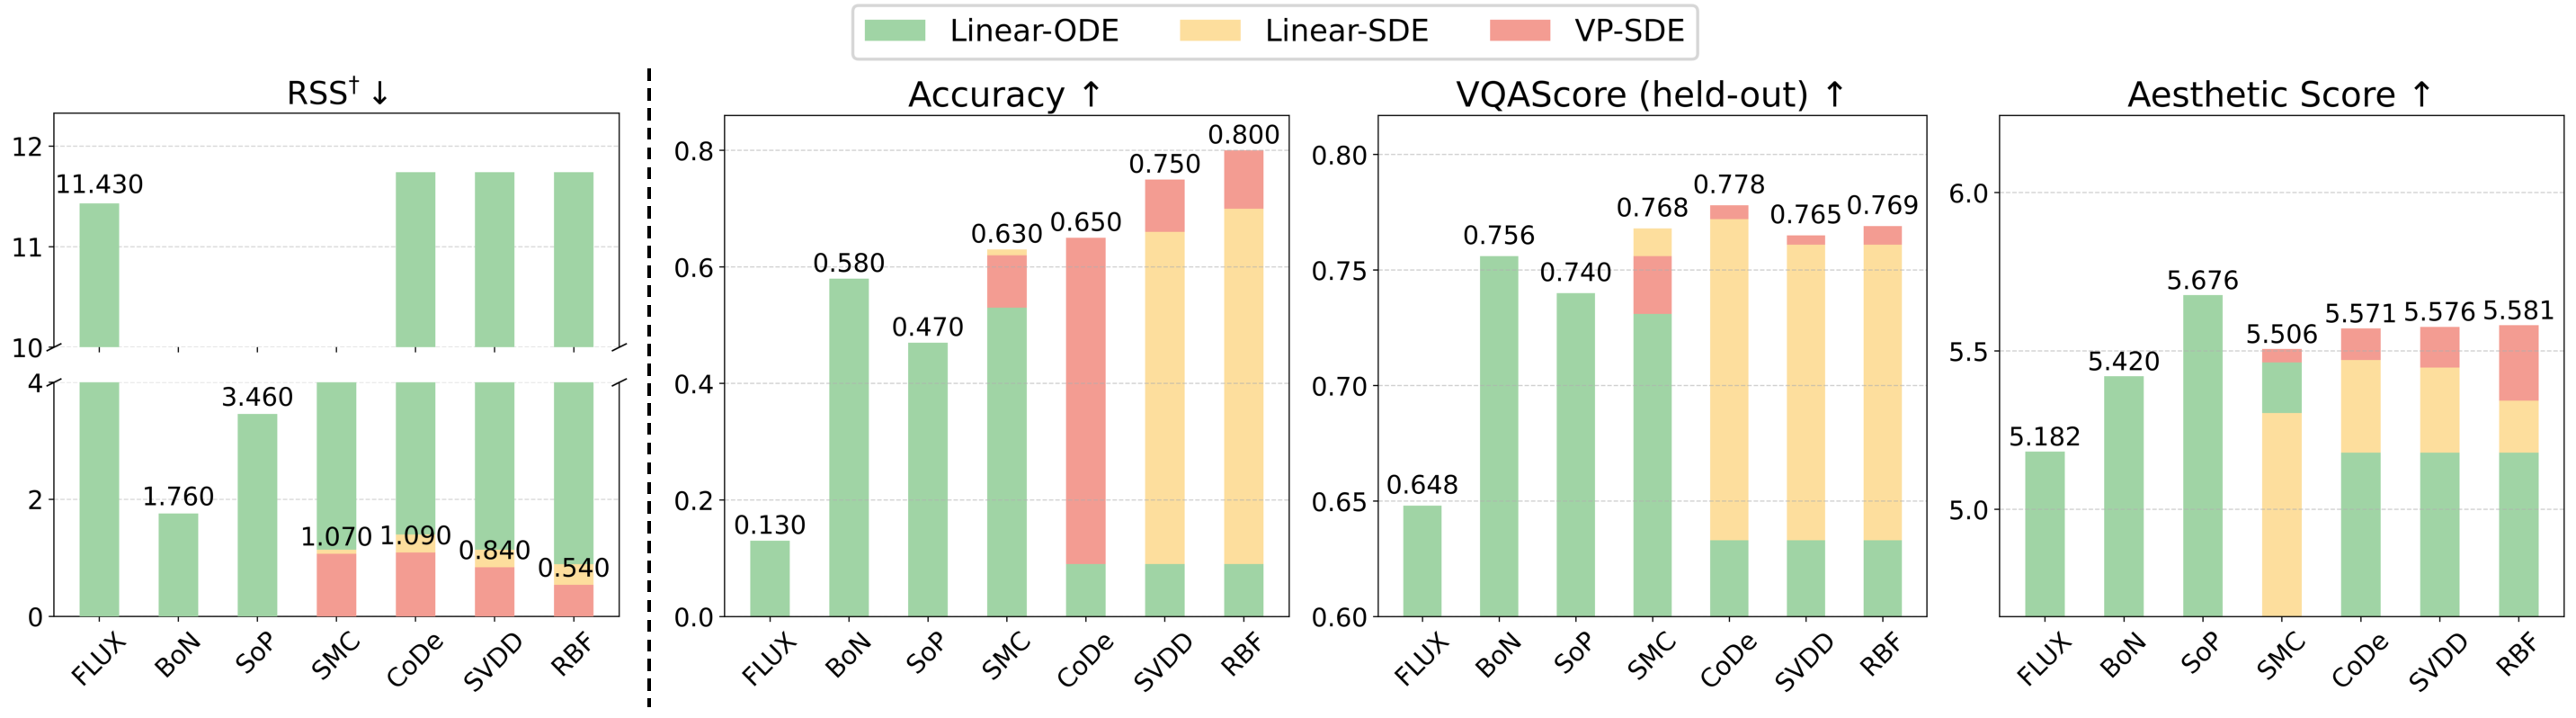
\includegraphics[width=1.0\linewidth]{Tables/quantity_bar_graph/quantity_bar_graph.pdf}
    \caption{\textbf{Quantitative results of quantity-aware image generation.} \textsuperscript{\textdagger} denotes the given reward, RSS~\cite{Liu:2024GroundingDINO}, with the y-axis truncated for better visualization (left). 
    We observe consistent performance improvements by converting {\color{YellowGreen}Linear-ODE} to {\color{Dandelion}{Linear-SDE}}, and {\color{Rhodamine}VP-SDE} for most cases.} 
    \label{fig:counting_main}
    \vspace{-0.75\baselineskip}
\end{figure}


% \begin{table*}[t!]
% \setlength{\tabcolsep}{1.5pt}
% \centering
% \scriptsize
% \renewcommand{\arraystretch}{1.2}
% \caption{\textbf{Quantitative results of quantity-aware image generation.} \textsuperscript{\textdagger} denotes the given reward used in inference-time scaling. The best result in the given and held-out reward is highlighted by \textbf{bold}, and the runner-up is \underline{underlined}. L.O., L.S., and V.S. indicate Linear-ODE, Linear-SDE, and VP-SDE.}
% \vspace{-0.5\baselineskip}
% \label{tab:counting_main}
% \newcolumntype{X}{>{\centering\arraybackslash}m{0.13\linewidth}}
% \newcolumntype{Y}{>{\centering\arraybackslash}m{0.065\linewidth}}
% \newcolumntype{W}{>{\centering\arraybackslash}m{0.045\linewidth}}

% \begin{tabular}{X | Y Y Y | W W W | W W W | W W W | W W W }
% \toprule
% \multirow{2}{*}{Metric} & 
% \multirow{1}{*}{\makecell{FLUX~\cite{BlackForestLabs:2024Flux}}} & 
% \multirow{1}{*}{BoN} & 
% \multirow{1}{*}{\makecell{SoP~\cite{Ma2025:SoP}}} & 
% \multicolumn{3}{c|}{SMC~\cite{Kim:2025DAS}} & 
% \multicolumn{3}{c|}{CoDe~\cite{Singh:2025CoDE}} & 
% \multicolumn{3}{c|}{SVDD~\cite{Li2024:SVDD}} & 
% \multicolumn{3}{c}{{\Oursbf{}} (Ours)} \\
% \cline{2-16}
% & \multicolumn{3}{c|}{L.O.} & L.O. & L.S. & V.S. & L.O. & L.S. & V.S. & L.O. & L.S. & V.S. & L.O. & L.S. & V.S. \\
% \hline
% \makecell{RSS\textsuperscript{\textdagger}\\\cite{Liu:2024GroundingDINO}~$\downarrow$} & 
% 11.430 & 1.760 & 3.460 & 
% 4.870 & 1.140 & 1.070 & 
% 11.740 & 1.400 & 1.090 & 
% 11.740 & 1.140 & \underline{0.840} & 
% 11.740 & 0.890 & \textbf{0.540} \\
% \hline
% \makecell{Accuracy\\\cite{Liu:2024GroundingDINO}~$\uparrow$} & 
% 0.130 & 0.580 & 0.470 & 
% 0.530 & 0.630 & 0.620 & 
% 0.090 & 0.650 & 0.650 & 
% 0.090 & 0.660 & \underline{0.750} & 
% 0.090 & 0.700 & \textbf{0.800} \\
% \hline
% \makecell{VQAScore\\\cite{Lin:2024CLIPFlanT5}~$\uparrow$ (held-out)} & 
% 0.648 & 0.756 & 0.740 & 
% 0.731 & 0.768 & 0.756 & 
% 0.633 & \underline{0.772} & \textbf{0.778} & 
% 0.633 & 0.761 & 0.765 & 
% 0.633 & 0.761 & 0.769 \\
% \hline
% \makecell{Aesthetic\\Score~\cite{Schuhmann:aesthetics}~$\uparrow$} & 
% 5.182 & 5.420 & 5.676 & 
% 5.464 & 5.304 & 5.506 & 
% 5.179 & 5.471 & 5.571 & 
% 5.179 & 5.447 & 5.576 & 
% 5.179 & 5.343 & 5.581 \\
% \bottomrule
% \end{tabular}
% \vspace{-0.5\baselineskip}
% \end{table*}




% previous version
% \begin{table*}[t!]
%     \setlength{\tabcolsep}{1.5pt}
%     \centering
%     \scriptsize
%     \newcommand{\good}[1]{\tiny{\textcolor{blue}{+#1\%}}}
%     \newcommand{\bad}[1]{\tiny{\textcolor{red}{-#1\%}}}
%     \caption{\textbf{Quantitative results of quantity-aware image generation.} \textsuperscript{\textdagger} denotes the given reward used in inference-time scaling. For particle-based sampling methods, the relative improvement in each cell is computed with respect to the Linear-ODE case. The best result in the given and held-out reward is highlighted by \textbf{bold}, and the runner-up is \underline{underlined}. L.O., L.S., and V.S. indicate Linear-ODE, Linear-SDE, and VP-SDE, respectively. \textsuperscript{*} denotes results with $50$ denoising steps.}
%     \vspace{-1.0\baselineskip}
%     \newcolumntype{X}{>{\centering\arraybackslash}m{0.095\linewidth}}
%     \newcolumntype{Y}{>{\centering\arraybackslash}m{0.045\linewidth}}
%     \newcolumntype{Z}{>{\centering\arraybackslash}m{0.05\linewidth}}
%     \newcolumntype{W}{>{\centering\arraybackslash}m{0.035\linewidth}}
%     \begin{tabular}{X | Y Y | Z Z | W W W | W Y Y | W Y Y | W Y Y | W Y Y }
%         \bottomrule
%         \multirow{4}{*}{\makecell{Metric}} & \multicolumn{4}{c|}{\textbf{Diffusion Model}} & \multicolumn{15}{c}{\textbf{Flow Model}} \\
%         \cline{2-20}
%         & \multirow{2}{*}{SD2} & \multirow{2}{*}{$\text{SD2}^{*}$} & \multicolumn{2}{c|}{SVDD~\cite{Li2024:SVDD}} & \multirow{2}{*}{FLUX} & \multirow{2}{*}{BoN} & \multirow{2}{*}{\makecell{SoP\\\cite{Ma2025:SoP}}} & \multicolumn{3}{c|}{\multirow{2}{*}{SMC~\cite{Kim:2025DAS}}} & \multicolumn{3}{c|}{\multirow{2}{*}{CoDe~\cite{Singh:2025CoDE}}} & \multicolumn{3}{c|}{\multirow{2}{*}{SVDD~\cite{Li2024:SVDD}}} & \multicolumn{3}{c}{\multirow{2}{*}{{\Oursbf{}} (Ours)}}\\
%         & & & SD2 & SD2$^{*}$ & & & & & & & & & & & & & & \\
%         % & \multirow{2}{*}{\makecell{SD}} & \multirow{2}{*}{\makecell{$\text{SD}^{*}$}} & \multicolumn{2}{c}{SVDD~\cite{Li2024:SVDD}} & \multirow{2}{*}{FLUX} & \multirow{2}{*}{BoN} & \multirow{2}{*}{SoP~\cite{Ma2025:SoP}} & \multirow{2}{*}{\multicolumn{3}{c|}}{\makecell{SMC \\ \cite{Kim:2025DAS}}} & \multirow{2}{*}{\multicolumn{3}{c|}{\makecell{CoDe \\ \cite{Singh:2025CoDE}}}} & \multirow{2}{*}{\multicolumn{3}{c|}{\makecell{SVDD\\\cite{Li2024:SVDD}}}} & \multirow{2}{*}{\multicolumn{3}{c}}{\makecell{{\Oursbf{}} (Ours)}} \\
        
%         % & \makecell{SD \\ \cite{Rombach:2022LDM}} & \makecell{$\text{SD}^{*}$ \\ \cite{Rombach:2022LDM}} & \makecell{SVDD \\ SD~\cite{Li2024:SVDD}} & \makecell{SVDD \\$\text{SD}^{*}$ \cite{Li2024:SVDD}} & \makecell{FLUX \\ \cite{BlackForestLabs:2024Flux}} & BoN & \makecell{SoP \\ \cite{Ma2025:SoP}} & \multicolumn{3}{c|}{\makecell{SMC \\ \cite{Kim:2025DAS}}} & \multicolumn{3}{c|}{\makecell{CoDe \\ \cite{Singh:2025CoDE}}} & \multicolumn{3}{c|}{\makecell{SVDD \\ \cite{Li2024:SVDD}}} & \multicolumn{3}{c}{\makecell{{\Oursbf{}} (Ours)}} \\
%         \cline{2-20}
%         & \multicolumn{2}{c|}{V.S.} & \multicolumn{2}{c|}{V.S.} & \multicolumn{3}{c|}{L.O.} & L.O. & L.S. & V.S. & L.O. & L.S. & V.S. & L.O. & L.S. & V.S. & L.O. & L.S. & V.S. \\
%         \hline
%         \makecell{RSS\textsuperscript{\textdagger} \cite{Liu:2024GroundingDINO} $\downarrow$} & 22.200 & 18.590 & 5.820 & 5.140 & 11.430 & 1.760 & 3.460 & 4.870 & \makecell{1.140 \\ \good{76.59}} & \makecell{1.070 \\ \good{78.03}} & 11.740 & \makecell{1.400 \\\good{88.07}} & \makecell{1.090 \\\good{90.72}} & 11.740 & \makecell{1.140 \\\good{90.29}} & \makecell{\underline{0.840} \\\good{92.84}} & 11.740 & \makecell{0.890 \\\good{92.42}} & \makecell{\textbf{0.540} \\\good{95.40}} \\
%         \hline
%         \makecell{Accuracy \\ \cite{Liu:2024GroundingDINO} $\uparrow$} & 0.020 & 0.050 & 0.470 & 0.470 & 0.130 & 0.580 & 0.470 & 0.530 & \makecell{0.630 \\\good{18.87}} & \makecell{0.620 \\\good{16.98}} & 0.090 & \makecell{0.650 \\\good{622.22}} & \makecell{0.650 \\\good{622.22}} & 0.090 & \makecell{0.660 \\\good{633.33}} & \makecell{\underline{0.750} \\\good{733.33}} & 0.090 & \makecell{0.700 \\\good{677.78}} & \makecell{\textbf{0.800} \\\good{788.89}} \\
%         \hline
%         \makecell{VQAScore~\cite{Lin:2024CLIPFlanT5} \\ $\uparrow$ (held-out)} & 0.523 & 0.532 & 0.617 & 0.648 & 0.648 & 0.756 & 0.740 & 0.731 & \makecell{0.768 \\\good{5.06}} & \makecell{0.756 \\\good{3.42}} & 0.633 & \makecell{\underline{0.772} \\\good{21.96}} & \makecell{\textbf{0.778} \\\good{22.91}} & 0.633 & \makecell{0.761 \\\good{20.22}} & \makecell{0.765 \\\good{20.85}} & 0.633 & \makecell{0.761 \\\good{20.22}} & \makecell{0.769 \\\good{21.48}} \\
%         \hline
%         \makecell{Aesthetic \\ Score~\cite{Schuhmann:aesthetics} $\uparrow$} & 5.060 & 5.223 & 4.983 & 5.081 & 5.182 & 5.420 & 5.676 & 5.464 & 5.304 & 5.506 & 5.179 & 5.471 & 5.571 & 5.179 & 5.447 & 5.576 & 5.179 & 5.343 & 5.581 \\
%         \toprule
%     \end{tabular}
%     \label{tab:counting_main}
%     \vspace{-0.25\baselineskip}
% \end{table*}


% previous version
% \begin{table*}[t!]
%     \setlength{\tabcolsep}{1.5pt}
%     \centering
%     \scriptsize
%     \newcommand{\good}[1]{\tiny{\textcolor{blue}{+#1\%}}}
%     \newcommand{\bad}[1]{\tiny{\textcolor{red}{-#1\%}}}
%     \caption{\textbf{Quantitative results of quantity-aware image generation.} \textsuperscript{\textdagger} denotes the given reward used in inference-time scaling. For particle-based sampling methods, the relative improvement in each cell is computed with respect to the Linear-ODE case. The best result in the given and held-out reward is highlighted by \textbf{bold}, and the runner-up is \underline{underlined}. L.O., L.S., and V.S. indicate Linear-ODE, Linear-SDE, and VP-SDE, respectively. \textsuperscript{*} denotes results with $50$ denoising steps.}
%     \vspace{-1.0\baselineskip}
%     \newcolumntype{X}{>{\centering\arraybackslash}m{0.095\linewidth}}
%     \newcolumntype{Y}{>{\centering\arraybackslash}m{0.045\linewidth}}
%     \newcolumntype{Z}{>{\centering\arraybackslash}m{0.05\linewidth}}
%     \newcolumntype{W}{>{\centering\arraybackslash}m{0.035\linewidth}}
%     \begin{tabular}{X | Y Y | Z Z | W W W | W Y Y | W Y Y | W Y Y | W Y Y }
%         \bottomrule
%         \multirow{4}{*}{\makecell{Metric}} & \multicolumn{4}{c|}{\textbf{Diffusion Model}} & \multicolumn{15}{c}{\textbf{Flow Model}} \\
%         \cline{2-20}
%         & \multirow{2}{*}{SD2} & \multirow{2}{*}{$\text{SD2}^{*}$} & \multicolumn{2}{c|}{SVDD~\cite{Li2024:SVDD}} & \multirow{2}{*}{FLUX} & \multirow{2}{*}{BoN} & \multirow{2}{*}{\makecell{SoP\\\cite{Ma2025:SoP}}} & \multicolumn{3}{c|}{\multirow{2}{*}{SMC~\cite{Kim:2025DAS}}} & \multicolumn{3}{c|}{\multirow{2}{*}{CoDe~\cite{Singh:2025CoDE}}} & \multicolumn{3}{c|}{\multirow{2}{*}{SVDD~\cite{Li2024:SVDD}}} & \multicolumn{3}{c}{\multirow{2}{*}{{\Oursbf{}} (Ours)}}\\
%         & & & SD2 & SD2$^{*}$ & & & & & & & & & & & & & & \\
%         % & \multirow{2}{*}{\makecell{SD}} & \multirow{2}{*}{\makecell{$\text{SD}^{*}$}} & \multicolumn{2}{c}{SVDD~\cite{Li2024:SVDD}} & \multirow{2}{*}{FLUX} & \multirow{2}{*}{BoN} & \multirow{2}{*}{SoP~\cite{Ma2025:SoP}} & \multirow{2}{*}{\multicolumn{3}{c|}}{\makecell{SMC \\ \cite{Kim:2025DAS}}} & \multirow{2}{*}{\multicolumn{3}{c|}{\makecell{CoDe \\ \cite{Singh:2025CoDE}}}} & \multirow{2}{*}{\multicolumn{3}{c|}{\makecell{SVDD\\\cite{Li2024:SVDD}}}} & \multirow{2}{*}{\multicolumn{3}{c}}{\makecell{{\Oursbf{}} (Ours)}} \\
        
%         % & \makecell{SD \\ \cite{Rombach:2022LDM}} & \makecell{$\text{SD}^{*}$ \\ \cite{Rombach:2022LDM}} & \makecell{SVDD \\ SD~\cite{Li2024:SVDD}} & \makecell{SVDD \\$\text{SD}^{*}$ \cite{Li2024:SVDD}} & \makecell{FLUX \\ \cite{BlackForestLabs:2024Flux}} & BoN & \makecell{SoP \\ \cite{Ma2025:SoP}} & \multicolumn{3}{c|}{\makecell{SMC \\ \cite{Kim:2025DAS}}} & \multicolumn{3}{c|}{\makecell{CoDe \\ \cite{Singh:2025CoDE}}} & \multicolumn{3}{c|}{\makecell{SVDD \\ \cite{Li2024:SVDD}}} & \multicolumn{3}{c}{\makecell{{\Oursbf{}} (Ours)}} \\
%         \cline{2-20}
%         & \multicolumn{2}{c|}{V.S.} & \multicolumn{2}{c|}{V.S.} & \multicolumn{3}{c|}{L.O.} & L.O. & L.S. & V.S. & L.O. & L.S. & V.S. & L.O. & L.S. & V.S. & L.O. & L.S. & V.S. \\
%         \hline
%         \makecell{RSS\textsuperscript{\textdagger} \cite{Liu:2024GroundingDINO} $\downarrow$} & 22.200 & 18.590 & 5.820 & 5.140 & 11.430 & 1.760 & 3.460 & 4.870 & \makecell{1.140 \\ \good{76.59}} & \makecell{1.070 \\ \good{78.03}} & 11.740 & \makecell{1.400 \\\good{88.07}} & \makecell{1.090 \\\good{90.72}} & 11.740 & \makecell{1.140 \\\good{90.29}} & \makecell{\underline{0.840} \\\good{92.84}} & 11.740 & \makecell{0.890 \\\good{92.42}} & \makecell{\textbf{0.540} \\\good{95.40}} \\
%         \hline
%         \makecell{Accuracy \\ \cite{Liu:2024GroundingDINO} $\uparrow$} & 0.020 & 0.050 & 0.470 & 0.470 & 0.130 & 0.580 & 0.470 & 0.530 & \makecell{0.630 \\\good{18.87}} & \makecell{0.620 \\\good{16.98}} & 0.090 & \makecell{0.650 \\\good{622.22}} & \makecell{0.650 \\\good{622.22}} & 0.090 & \makecell{0.660 \\\good{633.33}} & \makecell{\underline{0.750} \\\good{733.33}} & 0.090 & \makecell{0.700 \\\good{677.78}} & \makecell{\textbf{0.800} \\\good{788.89}} \\
%         \hline
%         \makecell{VQAScore~\cite{Lin:2024CLIPFlanT5} \\ $\uparrow$ (held-out)} & 0.523 & 0.532 & 0.617 & 0.648 & 0.648 & 0.756 & 0.740 & 0.731 & \makecell{0.768 \\\good{5.06}} & \makecell{0.756 \\\good{3.42}} & 0.633 & \makecell{\underline{0.772} \\\good{21.96}} & \makecell{\textbf{0.778} \\\good{22.91}} & 0.633 & \makecell{0.761 \\\good{20.22}} & \makecell{0.765 \\\good{20.85}} & 0.633 & \makecell{0.761 \\\good{20.22}} & \makecell{0.769 \\\good{21.48}} \\
%         \hline
%         \makecell{Aesthetic \\ Score~\cite{Schuhmann:aesthetics} $\uparrow$} & 5.060 & 5.223 & 4.983 & 5.081 & 5.182 & 5.420 & 5.676 & 5.464 & 5.304 & 5.506 & 5.179 & 5.471 & 5.571 & 5.179 & 5.447 & 5.576 & 5.179 & 5.343 & 5.581 \\
%         \toprule
%     \end{tabular}
%     \label{tab:counting_main}
%     \vspace{-0.25\baselineskip}
% \end{table*}





% \begin{table}[!t]
%     \setlength{\tabcolsep}{1.5pt}
%     \centering
%     \tiny
%     \newcommand{\good}[1]{\textcolor{red}{(+#1\%)}}
%     \newcommand{\bad}[1]{\textcolor{blue}{(-#1\%)}}
%     % \newcolumntype{X}{>{\columncolor{Yellow}\centering\arraybackslash}m{0.19\linewidth}}
%     \caption{\textbf{Quantitative results of quantity-aware image generation.} \textsuperscript{\textdagger} denotes the given reward used in inference time. For particle-based sampling methods, The relative improvement in each cell is computed with respect to the Linear-ODE. 
%     The best result in the detection score column is highlighted by \textbf{bold}, and the runner-up is \underline{underlined}.}
%     \label{tab:counting_main}
%     \newcolumntype{Z}{>{\centering\arraybackslash}m{0.155\linewidth}}
%     \begin{tabular}{Z Z | Z Z Z | Z }
%         \toprule
%         \multirow{2}{*}{\makecell{Search\\Algorithm}} & \multirow{2}{*}{\makecell{Sampling\\Method}} & 
%         \multicolumn{3}{c|}{Detection Score}
%         & \makecell{Image Quality} \\
%         \cline{3-6}
%         &  & \makecell{\textbf{\textbf{MSE}}\textsuperscript{\textdagger}~\cite{} $\downarrow$} & \makecell{\textbf{Accuracy}\textsuperscript{\textdagger}~\cite{} $\uparrow$} & \makecell{VQAScore~\cite{} $\uparrow$} & \makecell{Aesthetic \\ Score~\cite{} $\uparrow$} \\
%         % \multirow{2}{*}{\makecell{Search\\Algorithm}} & \multirow{2}{*}{\makecell{Sampling\\Method}} & \makecell{\textbf{Reward}} & \makecell{Text Alignment} & \makecell{Image Quality} \\
%         % \cline{3-5}
%         % &  & \makecell{\textbf{VQA Score}~\cite{} $\uparrow$} & \makecell{VQA Score \\ (Inst. BLIP)~\cite{} $\uparrow$} & \makecell{Aesthetic \\ Score~\cite{} $\uparrow$} \\
%         \hline
%         % ------------------------------------------------------------------------------------------
%         \multicolumn{1}{c}{SD~\cite{}} & VP-SDE & 22.200 & 0.020 & 0.523 & 5.060 \\
%         \hline
%         % ------------------------------------------------------------------------------------------
%         \multicolumn{1}{c}{SD~\cite{} x5} & VP-SDE & 18.590 & 0.050 & 0.532 & 5.223 \\
%         \hline
%         % ------------------------------------------------------------------------------------------
%         \multicolumn{1}{c}{SVDD (SD~\cite{})} & VP-SDE & 5.820 & 0.470 & 0.617 & 4.983\\
%         \hline
%         % ------------------------------------------------------------------------------------------
%         \multicolumn{1}{c}{SVDD (SD~\cite{} x5)} & VP-SDE & 5.140 & 0.470 & 0.648 & 5.081 \\
%         \hline
%         % ------------------------------------------------------------------------------------------
%         % ------------------------------------------------------------------------------------------
%         \multicolumn{6}{c}{\textbf{ODE-based Sampling}} \\
%         \hline
%         % ------------------------------------------------------------------------------------------
%         \multicolumn{1}{c}{Flux~\cite{}} & Linear-ODE & 11.430 & 0.130 & 0.648 & 5.182\\
%         \hline
%         % ------------------------------------------------------------------------------------------
%         \multirow{1}{*}{\makecell{BoN~\cite{}}} & Linear-ODE & 1.760 & 0.580 & 0.756 & 5.420 \\
%         \hline
%         % ------------------------------------------------------------------------------------------
%         \multirow{1}{*}{\makecell{SoP~\cite{}}} & Linear-ODE & 3.460 & 0.470 & 0.740 & 5.676 \\
%         % & VP-SDE & 3.080 \good{10.98} & 0.450 \bad{-4.26} & 0.756 \good{2.16} & 5.693 \\
%         \hline
%         % ------------------------------------------------------------------------------------------
%         % ------------------------------------------------------------------------------------------
%         \multicolumn{6}{c}{\textbf{Particle-based Sampling}} \\
%         \hline
%         % ------------------------------------------------------------------------------------------
%         \multirow{3}{*}{DAS} & Linear-ODE & 4.870 & 0.530 & 0.731 & 5.464 \\
%         & Linear-SDE & 1.140 \good{76.59} & 0.630 \good{18.87} & 0.768 \good{5.06} & 5.304 \\
%         & VP-SDE & 1.070 \good{78.03} & 0.620 \good{16.98} & 0.756 \good{3.42} & 5.506 \\
%         \hline
%         % ------------------------------------------------------------------------------------------
%         \multirow{3}{*}{\makecell{CoDe~\cite{}}} & Linear-ODE & 11.740 & 0.090 & 0.633 & 5.179 \\
%         & Linear-SDE & 1.400 \good{88.07} & 0.650 \good{622.22} & \underline{0.772} \good{21.96} & 5.471 \\
%         & VP-SDE & 1.090 \good{90.72} & 0.650 \good{622.22} & \textbf{0.778} \good{22.91} & 5.571 \\
%         \hline
%         % ------------------------------------------------------------------------------------------
%         \multirow{3}{*}{\makecell{SVDD~\cite{}}} & Linear-ODE & 11.740 & 0.090 & 0.633 & 5.179 \\
%         & Linear-SDE & 1.140 \good{90.29} & 0.660 \good{633.33} & 0.761 \good{20.22} & 5.447 \\
%         & VP-SDE & \underline{0.840} \good{92.84} & \underline{0.750} \good{733.33} & 0.765 \good{20.85} & 5.576 \\
%         \hline
%         % ------------------------------------------------------------------------------------------
%         \multirow{3}{*}{\Oursbf{}} & Linear-ODE & 11.740 & 0.090 & 0.633 & 5.179 \\
%         & Linear-SDE & 0.890 \good{92.42} & 0.700 \good{677.78} & 0.761 \good{20.22} & 5.343 \\
%         & VP-SDE & \textbf{0.540} \good{39.33} & \textbf{0.800} \good{14.29} & 0.769 \good{1.05} & 5.581 \\
%         \toprule
%     \end{tabular}
% \end{table}


% \begin{table}[!t]
%     \setlength{\tabcolsep}{2.9pt}
%     \tiny
%     \centering
%     \newcommand{\good}[1]{\textcolor{red}{(+#1\%)}}
%     \newcommand{\bad}[1]{\textcolor{blue}{(-#1\%)}}
%     \caption{\textbf{Quantitative results of quantity-aware image generation.} Superscript\textsuperscript{\textdagger} denotes the known reward. The relative improvement in each cell is computed with respect to the row directly above.}
%     \label{tab:counting_main}
%     % \vspace{-\baselineskip}
%     \newcolumntype{Z}{>{\centering\arraybackslash}m{0.07\textwidth}}
%     \begin{tabular}{Z Z | Z Z | Z Z Z}
%         \toprule
%         \multicolumn{2}{c|}{\tiny{Search Algorithm / Sampler}} & \makecell{MSE\textsuperscript{\textdagger} $\downarrow$} & \tiny{\makecell{Accuracy $\uparrow$}} & \tiny{\makecell{ Image\\Reward $\uparrow$ }} & \tiny{\makecell{Aesthetic \\ Score $\uparrow$}} \\
%         \midrule
%         % ------------------------------------------------------------------------------------------
%         \multicolumn{1}{c}{BoN (SD~\cite{})} & VP-SDE & - & - & - & - \\
%         \midrule
%         % ------------------------------------------------------------------------------------------
%         \multicolumn{1}{c}{BoN (SD~\cite{} x5)} & VP-SDE & - & - & - & - \\
%         \midrule
%         % ------------------------------------------------------------------------------------------
%         \multirow{1}{*}{\makecell{BoN~\cite{}}} & Linear-ODE & - & - & - & - \\
%         \midrule
%         % ------------------------------------------------------------------------------------------
%         \multirow{2}{*}{\makecell{SoP~\cite{}}} & Linear-SDE & - & - & - & - \\
%         & VP-SDE & - & - & - & - \\
%         \midrule
%         % ------------------------------------------------------------------------------------------
%         \multirow{3}{*}{SMC~\cite{}} & Linear-ODE & - & - & - & - \\
%         & Linear-SDE & - & - & - & - \\
%         & VP-SDE & - & - & - & - \\
%         \midrule
%         % ------------------------------------------------------------------------------------------
%         \multirow{3}{*}{\makecell{Block.\\BoK~\cite{}}} & Linear-ODE & - & - & - & - \\
%         & Linear-SDE & - & - & - & - \\
%         & VP-SDE & - & - & - & - \\
%         \midrule
%         % ------------------------------------------------------------------------------------------
%         \multirow{3}{*}{\makecell{BoK~\cite{}}} & Linear-ODE & - & - & - & - \\
%         & Linear-SDE & - & - & - & - \\
%         & VP-SDE & - & - & - & - \\
%         \midrule
%         % ------------------------------------------------------------------------------------------
%         \multirow{2}{*}{\Oursbf{}} & Linear-SDE & - & - & - & - \\
%         & VP-SDE & - & - & - & - \\
%         \bottomrule
%     \end{tabular}
% \end{table}

% ------------------------------------------------------------------------------------------------

% \begin{table}[!t]
%     \setlength{\tabcolsep}{2.9pt}
%     \small
%     \centering
%     \caption{Quantitative results in counting task using 100 prompts in T2I-CompBench~\cite{T2I-CompBench}.}
%     \label{tab:counting_main}
%     % \vspace{-\baselineskip}
%     \newcolumntype{Z}{>{\centering\arraybackslash}m{0.01\textwidth}}
%     \newcolumntype{Y}{>{\centering\arraybackslash}m{0.052\textwidth}}
%     % \newcolumntype{X}{>{\centering\arraybackslash}m{0.066\textwidth}}
%     \newcolumntype{X}{>{\centering\arraybackslash}m{0.086\textwidth}}
%     \begin{tabular}{Z X Y Y Y Y Y Y}
%         \toprule
%         \multicolumn{2}{c}{\textbf{Counting}} & MSE $\downarrow$ & Acc $\uparrow$ & \tiny{UniDet $\uparrow$} & \tiny{\makecell{VQA\\Score}}$\uparrow$ & \tiny{\makecell{Image\\Reward}}$\uparrow$ & \tiny{\makecell{Aesthetic\\Score $\uparrow$}} \\
%         \midrule
%         \multirow{2}{*}{\rotatebox{90}{SD}} & SVDD-10 & 5.820 & 0.470 & 0.505 & 0.617 & -0.006 & 4.983 \\
%         & SVDD-50 & 5.140 & 0.470 & 0.532 & 0.648 & 0.331 & 5.081 \\
%         \midrule
%         \multicolumn{2}{c}{BoN} & 1.760 & 0.580 & 0.600 & 0.756 & 0.895 & 5.420 \\
%         \midrule
%         \multirow{2}{*}{\rotatebox{90}{SoP}} & OT & 3.460 & 0.470 & 0.544 & 0.740 & 0.906 & 5.676 \\
%         & VP & 3.080 & 0.450 & 0.552 & 0.756 & 0.964 & 5.693 \\
%         \midrule
%         \multirow{3}{*}{\rotatebox{90}{SMC}} & OT-ODE & 4.870 & 0.530 & 0.586 & 0.731 & 0.895 & 5.464 \\
%         & OT-SDE & 1.140 & 0.630 & 0.607 & 0.768 & 0.956 & 5.304 \\
%         & VP-SDE & 1.070 & 0.620 & 0.625 & 0.756 & 0.996 & 5.506 \\
%         \midrule
%         \multirow{3}{*}{\rotatebox{90}{CoDe}} & OT-ODE & 11.740 & 0.090 & 0.485 & 0.633 & 0.465 & 5.179 \\
%         & OT-SDE & 1.400 & 0.650 & 0.598 & 0.772 & 0.811 & 5.471 \\
%         & VP-SDE & 1.090 & 0.650 & 0.568 & 0.778 & 0.938 & 5.571 \\
%         \midrule
%         \multirow{3}{*}{\rotatebox{90}{SVDD}} & OT-ODE & 11.740 & 0.090 & 0.485 & 0.633 & 0.465 & 5.179 \\
%         & OT-SDE & 1.140 & 0.660 & 0.603 & 0.761 & 0.812 & 5.447 \\
%         & VP-SDE & 0.840 & 0.750 & 0.574 & 0.765 & 0.927 & 5.576 \\
%         \midrule
%         \multirow{2}{*}{\rotatebox{90}{last}} &  OT-SDE & 0.890 & 0.700 & 0.621 & 0.761 & 0.959 & 5.343 \\
%         & VP-SDE & 0.540 & 0.800 & 0.622 & 0.769 & 0.902 & 5.581 \\
%         \midrule
%         \multirow{2}{*}{\rotatebox{90}{best}} &  OT-SDE & 0.670 & 0.740 & 0.626 & 0.785 & 1.166 & 5.613 \\
%         & VP-SDE & 0.430 & 0.840 & 0.631 & 0.782 & 1.167 & 5.668 \\
%         \bottomrule
%     \end{tabular}
% \end{table}
\begin{figure}[ht!]
\centering
{\scriptsize
\setlength{\tabcolsep}{0pt}
\renewcommand{\arraystretch}{0.0}
\newcolumntype{Y}{>{\centering\arraybackslash}m{0.025\textwidth}}
\newcolumntype{Z}{>{\centering\arraybackslash}m{0.155\textwidth}}
\newcolumntype{X}{>{\centering\arraybackslash}m{0.0002\textwidth}}

\begin{tabularx}{\textwidth}{Y Z Z Z X Y Z Z Z}
\toprule
& Linear-ODE & Linear-SDE & VP-SDE & & & Linear-ODE & Linear-SDE & VP-SDE \\
\midrule
& \multicolumn{3}{c}{\makecell{\textit{``Four balloons, one cup,}\\\textit{four desks, two dogs and four microwaves.''}}} & & 
& \multicolumn{3}{c}{\textit{\makecell{``Four candles, two balloons, one dog,\\two tomatoes and three helicopters.''}}} \\
\rotatebox{90}{\makecell{\scriptsize{SMC}~\cite{Kim:2025DAS}}} &
\includegraphics[width=0.15\textwidth]{Figures/counting_generation/collection_ode_sde_vp/SMC_ODE_0.jpg} &
\includegraphics[width=0.15\textwidth]{Figures/counting_generation/collection_ode_sde_vp/SMC_SDE_0.jpg} &
\includegraphics[width=0.15\textwidth]{Figures/counting_generation/collection_ode_sde_vp/SMC_VP-SDE_0.jpg} & & 
\rotatebox{90}{\makecell{\scriptsize{CoDe}~\cite{Singh:2025CoDE}}} &
\includegraphics[width=0.15\textwidth]{Figures/counting_generation/collection_ode_sde_vp/CoDe_ODE_1.jpg} &
\includegraphics[width=0.15\textwidth]{Figures/counting_generation/collection_ode_sde_vp/CoDe_SDE_1.jpg} &
\includegraphics[width=0.15\textwidth]{Figures/counting_generation/collection_ode_sde_vp/CoDe_VP-SDE_1.jpg} \\
\midrule
& \multicolumn{3}{c}{\textit{``Eight chairs.''}} & & 
& \multicolumn{3}{c}{\textit{\makecell{``One egg, three camels, four cars and four pillows.''}}} \\
\rotatebox{90}{\makecell{\scriptsize{SVDD}~\cite{Li2024:SVDD}}} &
\includegraphics[width=0.15\textwidth]{Figures/counting_generation/collection_ode_sde_vp/SVDD_ODE_0.jpg} &
\includegraphics[width=0.15\textwidth]{Figures/counting_generation/collection_ode_sde_vp/SVDD_SDE_0.jpg} &
\includegraphics[width=0.15\textwidth]{Figures/counting_generation/collection_ode_sde_vp/SVDD_VP-SDE_0.jpg} & & 
\rotatebox{90}{\makecell{\scriptsize{\Oursbf{}}}} &
\includegraphics[width=0.15\textwidth]{Figures/counting_generation/collection_ode_sde_vp/ours_ODE_2.jpg} &
\includegraphics[width=0.15\textwidth]{Figures/counting_generation/collection_ode_sde_vp/ours_SDE_2.jpg} &
\includegraphics[width=0.15\textwidth]{Figures/counting_generation/collection_ode_sde_vp/ours_VP-SDE_2.jpg} \\
\bottomrule
\end{tabularx}
}
\caption{
    \textbf{Qualitative results of quantity-aware image generation.}
    At inference-time, we guide generation using the negation of RSS~\cite{Liu:2024GroundingDINO} (Residual Sum of Squares) as the given reward, which measures the discrepancy between detected and target object counts. 
    SDE and interpolant conversion expands the search space to identify high reward samples. 
}
\label{fig:counting_methods_vp}
\vspace{-1.0\baselineskip}
\end{figure}
% \input{Figures/counting_generation/counting_methods_vp}

\vspace{-0.4\baselineskip}
\subsection{Quantity-Aware Image Generation}
\vspace{-0.3\baselineskip}
\label{sec:counting_generation}
\paragraph{Evaluation Metrics.} 
Here, the given reward is the negation of the Residual Sum of Squares (RSS) between the target counts and the detected object counts, computed using GroundingDINO~\cite{Liu:2024GroundingDINO} and SAM~\cite{Kirillov2023:SAM} (details in Appendix~\ref{sec:appendix_impl_details}). Additionally, we report object count accuracy, which evaluates whether all object quantities are correctly shown in the image. For the held-out reward, we report VQAScore measured with CLIP-FlanT5~\cite{Lin:2024CLIPFlanT5}. 
As in the previous application, we evaluate the quality of the generated images using the aesthetic score~\cite{Schuhmann:aesthetics}. 

\vspace{-0.5\baselineskip}
\paragraph{Results.} The quantitative and qualitative results are presented in Fig.~\ref{fig:counting_main} and Fig.~\ref{fig:counting_methods_vp}, respectively. 
The trend in Fig.~\ref{fig:counting_main} align with those in Sec.~\ref{sec:compositional_generation}, demonstrating that SDE conversion and interpolant conversion synergistically enhance the identification of high-reward samples. 
Notably, particle sampling methods with Linear-SDE already outperform Linear-ODE-based methods (BoN and SoP~\cite{Ma2025:SoP}), while interpolant conversion further improves accuracy, achieving a $4\sim6 \times$ improvement over the base model~\cite{BlackForestLabs:2024Flux}. 
Our \Ours{} achieves the highest accuracy, outperforming all other particle sampling methods. 
Qualitatively, Fig.~\ref{fig:counting_methods_vp} shows that SDE and interpolant conversion effectively identify high-reward samples that accurately match the specified object categories and quantities. Additional qualitative comparisons of the inference-time scaling methods are provided in Appendix~\ref{sec:appendix_quali_search_alg}. 

% ===================================================================================================
